\documentclass[11pt]{article}

% Page format
\usepackage[margin=1in]{geometry}

% Math packages and custom commands 
\usepackage{framed, tikz}
\usepackage[utf8]{inputenc}
\usepackage{mathtools,amsthm}
\usepackage{enumitem,amssymb}
\usepackage{bbm}
\usepackage{hyperref}
\definecolor{shadecolor}{gray}{0.9}


\newtheoremstyle{case}{}{}{}{}{}{:}{}{}
\theoremstyle{case}
\newtheorem{case}{Case}
\DeclareMathOperator{\R}{\mathbb{R}}
\DeclareMathOperator{\E}{\mathbb{E}}
\DeclareMathOperator{\Var}{\text{Var}}
\DeclareMathOperator{\Cov}{\text{Cov}}
\newcommand{\bvec}[1]{\mathbf{#1}}
\renewcommand{\P}{\mathbb{P}}
\newcommand{\norm}[2][2]{\| #2\|}
\newcommand{\note}[1]{\noindent{[\textbf{NOTE:} #1]}}
\newcommand{\hint}[1]{\noindent{[\textbf{HINT:} #1]}}
\newcommand{\recall}[1]{\noindent{[\textbf{RECALL:} #1]}}

\DeclareMathOperator*{\argmin}{arg\,min}
\DeclareMathOperator*{\argmax}{arg\,max}


\begin{document}

\begin{center}
{\Large CSCE 790-003, Spring 2022 \\ Assignment 3}

\begin{tabular}{rl}
Username: & [your email username] \\
Name: & [your first and last name] \\
\end{tabular}
\end{center}
By turning in this assignment, I agree by the honor code of USC Columbia.

\paragraph{Submission.}
You need to submit the following files to Blackboard:
\begin{itemize}
    \item A pdf file named as assignment3\_$\langle username \rangle$.pdf, where you replace $\langle username \rangle$ with your email username. This pdf file contains your answers to the written problems, including problems 1 and 2.6.
    \item A zip file named as assignment3\_$\langle username \rangle$.zip, where you replace $\langle username \rangle$ with your email username. This zip file contains the whole directory of \texttt{starter\_code\_torch} to reproduce your result for problem 2.6.
\end{itemize}

\section{Per-trajectory REINFORCE [25 pt]}
In class, the policy gradient expressions we derived are ``per-step'', that is, the gradient estimator can be calculated for every step $t$ of a sampled trajectory. For example, the REINFORCE estimator is $\nabla_\theta \log \pi_\theta(a_t|s_t) \cdot G_t$.
In this problem, we will derive the ``per-trajectory'' REINFORCE.

Still, we consider a stochastic policy parameterized by $\theta$, $\pi_\theta(\cdot|s)$. The initial state is fixed to be some state $s_o$.
Let $\tau=(s_0, a_0, r_0, s_1, a_1, r_1,...)$ denote the state-action-reward trajectory.
The probability distribution over trajectories under policy $\pi_\theta$ can be expressed as
\begin{align*}
    p^{\pi_\theta}(\tau) = \pi_\theta(a_0|s_0)p(s_1|s_0,a_0)\pi_\theta(a_1|s_1)...
\end{align*}
assuming the reward function is deterministic, $r_t = R(s_t, a_t)$.
The discounted total reward of trajectory $\tau$ is denoted as
\begin{align*}
    G(\tau) := \sum_{t=0}^{H-1} \gamma^t r_t
\end{align*}
where horizon $H$ can be finite or infinite.

For per-trajectory REINFORCE, we start by decomposing the objective into trajectories, i.e. $V^{\pi_\theta}(s_0) = \sum_\tau [p^{\pi_\theta}(\tau) \cdot G(\tau) ]$.

\begin{enumerate}[label=(\alph*)]
    \item  Show that the policy gradient can be expressed as 
    \begin{align*}
        \nabla_\theta V^{\pi_\theta}(s_0) =& \nabla_\theta \sum_\tau [p^{\pi_\theta}(\tau) \cdot G(\tau) ]\\ 
        =& \mathbb{E}_{\tau\sim p^\pi(\tau)} \left[ G(\tau) \cdot \nabla_\theta \log\pi_\theta(\tau) \right].
    \end{align*}
    where $\log\pi_\theta(\tau) := \sum_{t=0}^{H-1} \log\pi_\theta(a_t|s_t)$
    Accordingly, the gradient estimator $G(\tau) \cdot \log\pi_\theta(\tau)$ is called the ``per-trajectoy'' REINFORCE.
    
    \underline{HINT:}
    \begin{align*}
        \nabla_\theta \sum_\tau [ p^{\pi_\theta}(\tau) \cdot G(\tau) ] = \sum_\tau [\nabla_\theta  p^{\pi_\theta}(\tau) \cdot G(\tau) ] = \sum_\tau [p^{\pi_\theta}(\tau) \nabla_\theta \log p^{\pi_\theta}(\tau) \cdot G(\tau) ]
    \end{align*}
    \begin{shaded}
			$\tau=(s_0, a_0, r_0, s_1, a_1, r_1,...)$, $p^{\pi_\theta}(\tau) = \pi_\theta(a_0|s_0)p(s_1|s_0,a_0)\pi_\theta(a_1|s_1)..., G(\tau) := \sum_{t=0}^{H-1} \gamma^t R(s_t, a_t)$
\begin{align*}
        V^{\pi_\theta}(s_0) =&\E _{\theta} [ G(s_0)] = \sum_\tau [p^{\pi_\theta}(\tau) \cdot G(\tau) ]\\ 
				\nabla_\theta 	V^{\pi_\theta}(s_0) = & \sum_\tau [\nabla_\theta  p^{\pi_\theta}(\tau) \cdot G(\tau) ]\\
    = & \sum_\tau [p^{\pi_\theta}(\tau) \nabla_\theta [\log p^{\pi_\theta}(\tau)] \cdot G(\tau) ]\\
	  = & \sum_\tau [p^{\pi_\theta}(\tau) \nabla_\theta \log [  \pi_\theta(a_0|s_0)p(s_1|s_0,a_0)\pi_\theta(a_1|s_1)... ] \cdot G(\tau) ]\\
		= & \sum_\tau [p^{\pi_\theta}(\tau) \nabla_\theta [  \log \pi_\theta(a_0|s_0) + \log p(s_1|s_0,a_0) + \log \pi_\theta(a_1|s_1) + ... ] \cdot G(\tau) ]\\
\end{align*}

As the reward function is deterministic, we have $\log p(s_{t+1}|s_{t},a_{0}) = \log 1 = 0 $ at all $t$:
\begin{align*}
\nabla_\theta 	V^{\pi_\theta}(s_0) = & \sum_\tau [p^{\pi_\theta}(\tau) \nabla_\theta [ \sum_{t = 0}^{H-1} \log \pi_\theta(a_t|s_t) ] \cdot G(\tau) ]\\
= & \sum_\tau p^{\pi_\theta}(\tau) [\nabla_\theta \log\pi_\theta(\tau) \cdot G(\tau) ]\\
=& \mathbb{E}_{\tau\sim p^\pi(\tau)} \left[ G(\tau) \cdot \nabla_\theta \log\pi_\theta(\tau) \right]\\
\end{align*}
\end{shaded}
    
    \item A baseline can be introduced to reduce the variance for the ``per-trajectoy'' REINFORCE. Specifically, we consider using a constant baseline $b\in\mathbb{R}$, which introduces no bias:
    \begin{align*}
        \nabla_\theta V^{\pi_\theta}(s_0) 
        =& \mathbb{E}_{\tau\sim p^{\pi_\theta}(\tau)} \left[ (G(\tau)-b ) \nabla_\theta \log\pi_\theta(\tau) \right].
    \end{align*}
    For simplicity, let's consider the 1-d case where $\theta \in \mathbb{R}$.
    We now look at the variance of the gradient estimator $\widehat{g}:=(G(\tau) - b) \nabla_\theta\log \pi_\theta(\tau) \in \mathbb{R}$.
    What's the optimal baseline that minimizes the variance of $\widehat{g}$?
    
    \underline{HINT:} Express the variance as $Var[\widehat{g}] = \mathbb{E}[\widehat{g}^2] - (\mathbb{E}[\widehat{g}])^2$. Then view $Var[\widehat{g}]$ as a function of baseline $b$; find its minimizer $b^*$. 
    \begin{shaded}
\begin{align*}
   \Var(\nabla_{\theta} V^{\pi_\theta}(s_0) ) = & \Var \{ \mathbb{E}_{\tau\sim p^{\pi_\theta}(\tau)} [ (G(\tau)-b) \nabla_{\theta} \log \pi_\theta (\tau)] \}\\
	= & \Var \{ \sum_\tau p^{\pi_\theta}(\tau) [ (G(\tau)-b) \nabla_{\theta} \log \pi_\theta (\tau)] \}\\
	= &  \sum_\tau p^{\pi_\theta}(\tau) ^2 \Var \{  [ (G(\tau)-b) \nabla_{\theta} \log \pi_\theta (\tau)] \} \\
\end{align*}

Let $\widehat{g}:=(G(\tau) - b) \nabla_\theta\log \pi_\theta(\tau) \in \mathbb{R}$,

\begin{align*}
   \Var(\nabla_{\theta} V^{\pi_\theta}(s_0) ) = & \sum_\tau p^{\pi_\theta}(\tau)^2 \{ \E (\hat{g}^2) - \E (\hat{g})^2 \}
\end{align*}

Let $\frac{d}{d b} \{\sum_\tau p^{\pi_\theta}(\tau)^2 [\E (\hat{g}^2) - \E (\hat{g})^2] \} =\sum_\tau p^{\pi_\theta}(\tau)^2 \frac{d}{d b} \{ \E ( \hat{g}^2) - \E (\hat{g})^2  \} = 0$. As $b$ introduce no bias and is a constant:

\begin{align*}
&\sum_\tau p^{\pi_\theta}(\tau) b \nabla_{\theta} \log \pi_\theta (\tau) = b \sum_\tau p^{\pi_\theta}(\tau) \nabla_{\theta} \log \pi_\theta (\tau) = 0\\
 & \E (\frac{d}{d b} \hat{g})  = \sum_\tau - p^{\pi_\theta}(\tau) \nabla_{\theta} \log \pi_\theta (\tau) = 0
\end{align*}

Then we have:

\begin{align*}
 \frac{d}{d b} \{ \Var(\nabla_{\theta} V^{\pi_\theta}(s_0) ) \} 
 = & \sum_\tau p^{\pi_\theta}(\tau)^2 \frac{d}{d b}\E ( \hat{g}^2) - \sum_\tau p^{\pi_\theta}(\tau)^2 \frac{d}{d b}\E (\hat{g})^2\\
 = & \sum_\tau p^{\pi_\theta}(\tau)^2 \E (\frac{d}{d b} \hat{g}^2) - \sum_\tau p^{\pi_\theta}(\tau)^2 \E (\frac{d}{d b} \hat{g})^2\\
=& \sum_\tau p^{\pi_\theta}(\tau)^2 \E ( 2 \hat{g} \frac{d \hat{g}}{d b} ) = 0
\end{align*}

$$- 2 \sum_\tau p^{\pi_\theta}(\tau)^2 \{  [ (G(\tau)-b) \nabla_{\theta} \log \pi_\theta (\tau)] \nabla_{\theta} \log \pi_\theta (\tau) \} = 0 $$

$$- 2 \sum_\tau p^{\pi_\theta}(\tau)^2 G(\tau) [\nabla_{\theta} \log \pi_\theta (\tau)]^2 + 2 \sum_\tau p^{\pi_\theta}(\tau)^2 b [\nabla_{\theta} \log \pi_\theta (\tau)]^2= 0 $$

$$  b \sum_\tau p^{\pi_\theta}(\tau)^2 [\nabla_{\theta} \log \pi_\theta (\tau)]^2 =  \sum_\tau p^{\pi_\theta}(\tau)^2 G(\tau) [\nabla_{\theta} \log \pi_\theta (\tau)]^2 $$

$$b = \frac{\sum_\tau p^{\pi_\theta}(\tau)^2 G(\tau) [\nabla_{\theta} \log \pi_\theta (\tau)]^2}{\sum_\tau p^{\pi_\theta}(\tau)^2 [\nabla_{\theta} \log \pi_\theta (\tau)]^2}$$
    \end{shaded}
\end{enumerate}

\newpage
\section{Implementing Policy Gradient [75 pt]}
This problem is adapted from Emma Brunskill's course.
The starter code is in folder \texttt{starter\_code\_torch}.

The goal of this problem is to experiment with policy gradient and its variants, including variance reduction methods. Your goals will be to set up policy gradient for both continuous and discrete environments, and implement a neural network baseline for variance reduction. The framework for the policy gradient algorithm is setup in \texttt{main.py}, and everything that you need to implement is in the files \texttt{network\_utils.py}, \texttt{policy.py}, \texttt{policy\_gradient.py} and \texttt{baseline\_network.py}. The file has detailed instructions for each implementation task, but an overview of key steps in the algorithm is provided here.

\subsection{REINFORCE}
Recall the policy gradient theorem (finite horizon with $\gamma=1$): the gradient of the policy performance, denoted as $\nabla_\theta J(\theta)$, can be expressed as 
\[ \nabla_\theta J(\theta) = \mathbb E_{\tau \sim \pi_\theta} \left[\sum_t \nabla_\theta \log\pi_\theta(a_t|s_t) Q^{\pi_\theta} (s_t,a_t) \right], \]
where $\tau$ is a trajectory.
REINFORCE is a Monte Carlo policy gradient algorithm, so we will be using the sampled returns $G_t$ as unbiased estimates of $Q^{\pi_\theta}(s,a)$. 
The REINFORCE estimator can be expressed as the gradient of the following objective function (e.g., for automatic differentiation):
\[ J(\theta) = \frac{1}{\sum _i T_i} \sum_{i=1}^{|D|} \sum_{t=1}^{T_i} \log(\pi_\theta(a^i_t|s^i_t)) G^i_t \]
where $D$ is the set of all trajectories collected by policy $\pi_\theta$, and $\tau^i =(s^i_1, a^i_1, r^i_1, s^i_2, \dots, s^i_{T_i}, a^i_{T_i}, r^i_{T_i})$ is trajectory $i$ (using 1-based indexing for $t$).

\subsection{Baseline}
One difficulty of training with the REINFORCE algorithm is that the Monte Carlo sampled return(s) $G_t$ can have high variance. To reduce variance, we subtract a baseline $b_{\phi}(s)$ from the estimated returns when computing the policy gradient. A good baseline is the state value function, $V^{\pi_\theta}(s)$, which requires a training update to $\phi$ to minimize the following mean-squared error loss:
\[ L_{\text{MSE}}(\phi) = \frac{1}{\sum _i T_i} \sum_{i=1}^{|D|} \sum_{t=1}^{T_i} (b_{\phi}(s^i_t) - G^i_t)^2\]

\subsection{Advantage Normalization}

After subtracting the baseline, we get the following new objective function:

\[ J(\theta) = \frac{1}{\sum _i T_i} \sum_{i=1}^{|D|} \sum_{t=1}^{T_i} \log(\pi_\theta(a^i_t|s^i_t)) \hat{A}^i_t \]

where

\[\hat{A}^i_t = G^i_t - b_{\phi}(s^i_t)\]

A second variance reduction technique is to normalize the computed advantages, $\hat{A}^i_t$, so that they have mean $0$ and standard deviation $1$. From a theoretical perspective, we can consider centering the advantages to be simply adjusting the advantages by a constant baseline, which does not change the policy gradient. Likewise, rescaling the advantages effectively changes the learning rate by a factor of $1/\sigma$, where $\sigma$ is the standard deviation of the empirical advantages.

\subsection{Functions to Implement}
The functions that you need to implement in \texttt{network\_utils.py}, \texttt{policy.py}, \texttt{policy\_gradient.py}, and \texttt{baseline\_network.py} are enumerated here. Detailed instructions for each function can be found in the comments in each of these files.

Note: The ``batch size'' for all the arguments is $\sum _i T_i$ since we already flattened out all the episode observations, actions, and rewards for you.

In \texttt{network\_utils.py},
\begin{itemize}
\item \texttt{build\_mlp}
\end{itemize}

In \texttt{policy.py},
\begin{itemize}
\item \texttt{BasePolicy.act}
\item \texttt{CategoricalPolicy.action\_distribution}
\item \texttt{GaussianPolicy.\_\_init\_\_}
\item \texttt{GaussianPolicy.std}
\item \texttt{GaussianPolicy.action\_distribution}
\end{itemize}

In \texttt{policy\_gradient.py},
\begin{itemize}
\item \texttt{PolicyGradient.init\_policy}
\item \texttt{PolicyGradient.get\_returns}
\item \texttt{PolicyGradient.normalize\_advantage}
\item \texttt{PolicyGradient.update\_policy}
\end{itemize}

In \texttt{baseline\_network.py},
\begin{itemize}
\item \texttt{BaselineNetwork.\_\_init\_\_}
\item \texttt{BaselineNetwork.forward}
\item \texttt{BaselineNetwork.calculate\_advantage}
\item \texttt{BaselineNetwork.update\_baseline}
\end{itemize}

\subsection{Testing}
We have provided some basic tests to sanity check your implementation. \textbf{Please note that the tests are not comprehensive, and passing them does not guarantee a correct implementation}. Use the following command to run the tests:
\begin{verbatim}
python run_basic_tests.py
\end{verbatim}
You can also add additional tests of your own design in \texttt{tests/test\_basic.py}.

\subsection{Getting Plots}
The general form for running your policy gradient implementation is as follows:
\begin{verbatim}
python main.py --env-name ENV --seed SEED --no-baseline
\end{verbatim}
if not using a baseline, or
\begin{verbatim}
python main.py --env-name ENV --seed SEED --baseline
\end{verbatim}
if using a baseline. Here \texttt{ENV} can be \texttt{cartpole}, \texttt{pendulum}, or \texttt{cheetah}, and \texttt{SEED} should be a positive integer.

For an environment, choose 3 random seeds and run the algorithm both without baseline and with baseline. Then plot the results using
\begin{verbatim}
python plot.py --env-name ENV --seeds SEEDS
\end{verbatim}
where \texttt{SEEDS} should be a comma-separated list of seeds which you want to plot (e.g. \texttt{--seeds 1,2,3}).

\textbf{ Since \texttt{pendulum} and \texttt{cheetah} require mujoco license, you are not required to run them. Even if you run them, exclude their plots from your writeup. Please include the plot for \texttt{cartpole} only in your writeup, and comment on whether or not you observe improved performance when using a baseline.}

We have the following expectations about performance:
\begin{itemize}
    \item cartpole: Should reach the max reward of 200 (although it may not stay there)
    \item pendulum: Should reach the max reward of 1000 (although it may not stay there)
    \item cheetah: Should reach at least 200 (Could be as large as 950)
\end{itemize}

\begin{shaded}
Baseline:\\
\begin{minipage}{1\linewidth}\centering
	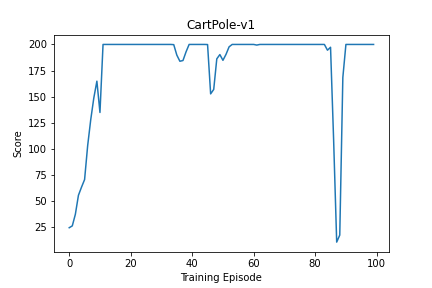
\includegraphics[width=0.315\linewidth]{./starter_code_torch/code/results/CartPole-v1-baseline-seed=1/scores.png}
	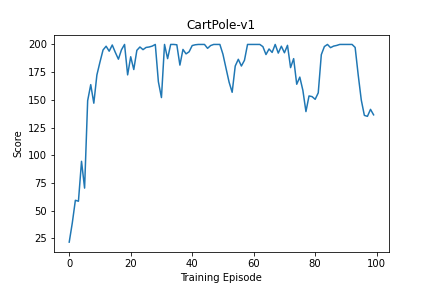
\includegraphics[width=0.315\linewidth]{./starter_code_torch/code/results/CartPole-v1-baseline-seed=2/scores.png}
	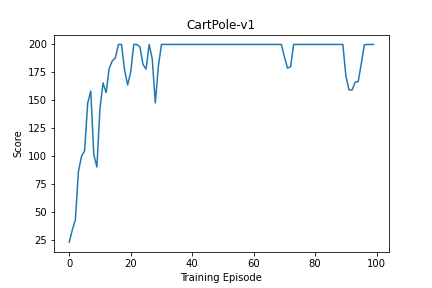
\includegraphics[width=0.315\linewidth]{./starter_code_torch/code/results/CartPole-v1-baseline-seed=3/scores.png}
\end{minipage}
No baseline:\\
\begin{minipage}{1\linewidth}\centering
	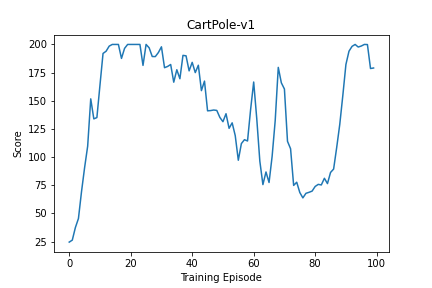
\includegraphics[width=0.315\linewidth]{./starter_code_torch/code/results/CartPole-v1-no_baseline-seed=1/scores.png}
	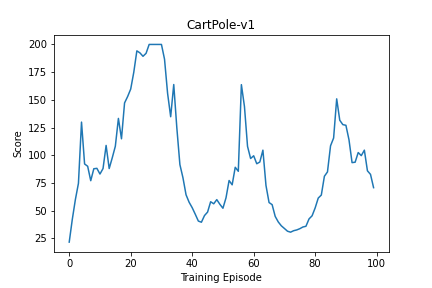
\includegraphics[width=0.315\linewidth]{./starter_code_torch/code/results/CartPole-v1-no_baseline-seed=2/scores.png}
	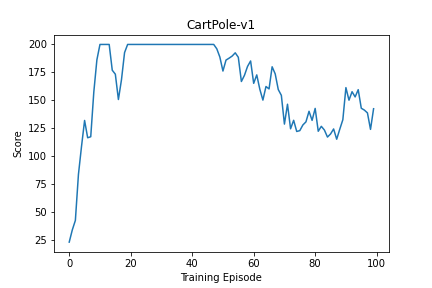
\includegraphics[width=0.315\linewidth]{./starter_code_torch/code/results/CartPole-v1-no_baseline-seed=3/scores.png}
\end{minipage}
\end{shaded}

\newpage
\section{Regret Analysis of Explore-Then-Commit for MAB [25 pt]}
Consider a multi-armed bandit (MAB) specified by
\begin{itemize}
    \item $K$ arms with $[0,1]$-bounded reward  distributions $\nu_1,...,\nu_K\in\Delta([0,1])$
    \item Game length $T$
\end{itemize}
We use the following notations:
\begin{itemize}
    \item $\mu_i:=\E_{X\sim\nu_i}[X]$, the true mean of arm $i$ 
    \item $i^*:=\argmax_i \mu_i$, the best arm $i^*$
    \item $\Delta_i:=\mu_{i^*} -\mu_{i} $, the gap of arm $i$
    \item $I_t\in\{1,...,K\}$ is the arm pulled at round $t$;
    $X_t\sim\nu_{I_t}$ is the reward received at round $t$
    \item $N_{i,t}:=\sum_{s=1}^{t}\mathbbm{1}[I_s=i]$, number of pulls of arm $i$ by round $t$, where $\mathbbm{1}[E]$ is the indicator function of event $E$
    \item $\hat{\mu}_{i,t}:=\frac{1}{N_{i,t}}\sum_{s=1}^{t}X_s \cdot \mathbbm{1}[I_s=i]$, empirical mean of arm $i$ by round $t$
\end{itemize}
Consider the Explore-Then-Commit algorithm with exploration parameter $M$:
\begin{enumerate}
    \item For $t=1,...,MK$, pull each arm $M$ times.
    \item For $t=MK+1,...,T$, pull the empirically best arm $\hat{i}:=\argmax_j \hat{\mu}_{j, MK}$.
\end{enumerate}
Prove that its pseudo-regret is bounded as 
\begin{align*}
    \overline{R_T}:=\sum_i \Delta_i\E[N_{i,T}] 
    \leq \sum_i \Delta_i \left(M+2(T-MK)e^{\frac{-M\Delta_i^2}{2}}\right)
\end{align*}

\underline{Hint:}
Since 
\begin{align*}
    N_{i,T} =& M + (T-MK)\cdot \mathbbm{1}[i=\argmax_j \hat{\mu}_{j, MK}] \\
    \E[N_{i,T}] =& M + (T-MK)\cdot \Pr(i=\argmax_j \hat{\mu}_{j, MK})
\end{align*}
It suffices to show that for any given suboptimal arm $i: \Delta_i>0$, $\Pr(i=\argmax_j \hat{\mu}_{j, MK})\leq 2e^{\frac{-M\Delta_i^2}{2}}$. We show this next, using $\hat{\mu}_i$ as shorthand for $\hat{\mu}_{i,MK}$.

By Hoeffding's bound, for any given arm $j$,
\begin{align*}
    &\Pr(\hat{\mu}_j-\mu_j \geq\epsilon)\leq e^{-2\epsilon^2M}\\
    &\Pr(\hat{\mu}_j-\mu_j \leq - \epsilon)\leq e^{-2\epsilon^2M}
\end{align*}
For any given suboptimal arm $i: \Delta_i>0$, if we set $\epsilon=\Delta_i/2$ for $j\in\{i, i^*\}$, then arm $i$ will be favored over optimal arm $i^*$ with low probability. 

\begin{shaded}
It is obvious that for the operations: $t=1,...,MK$, pull each arm $M$ times, then for $t=MK+1,...,T$, pull the empirically best arm $\hat{i}:=\argmax_j \hat{\mu}_{j, MK}$:

\begin{align*}
    N_{i,T} =& \sum_{s=1}^{T}\mathbbm{1}[I_s=i] =  M + (T-MK)\cdot \mathbbm{1}[i=\argmax_j \hat{\mu}_{j, MK}] \\
    \E[N_{i,T}] =& M + (T-MK)\cdot \Pr(i=\argmax_j \hat{\mu}_{j, MK})
\end{align*}

For any given suboptimal arm $i: \Delta_i>0$. By Hoeffding's bound, for any given arm $j$,

\begin{align*}
    &\Pr(\hat{\mu}_j-\mu_j \geq\epsilon)\leq e^{-2\epsilon^2M}\\
    &\Pr(\hat{\mu}_j-\mu_j \leq - \epsilon)\leq e^{-2\epsilon^2M}
\end{align*}

For any given suboptimal arm $i: \Delta_i>0$, if we set $\epsilon=\Delta_i/2$ for $j\in\{i, i^*\}$, then  using $\hat{\mu}_i$ as shorthand for $\hat{\mu}_{i,MK}$

\begin{align*}
   & \Pr(i=\argmax_j \hat{\mu}_{j, MK}) = \Pr(\hat{\mu}_{i, MK} \geq \max_{i \neq j} \hat{\mu}_{j, MK}) \\
\leq &  \Pr(\hat{\mu}_{i, MK} \geq \hat{\mu}_{i_*, MK}) = \Pr(\hat{\mu}_{i, MK} - \hat{\mu}_{i_*, MK} + \mu_{i^*} -\mu_{i} \geq \mu_{i^*} -\mu_{i} )\\
= & \Pr(\hat{\mu}_{i, MK} - \hat{\mu}_{i_*, MK} - \mu_{i^*} + \mu_{i} \geq - \mu_{i^*} + \mu_{i} )\\
\leq &  \Pr( - \mu_{i^*} + \mu_{i} \leq 2 \hat{\mu}_i-2 \mu_i \leq \mu_{i^*} -\mu_{i})\\
 = &	\Pr( -\Delta_i/2 \leq \hat{\mu}_i-\mu_i \leq \Delta_i/2) \\
 = & \Pr(\hat{\mu}_i-\mu_i \geq \Delta_i/2) + \Pr(\hat{\mu}_i\mu_i \leq - \Delta_i/2)\\
\leq & e^{-2(\Delta_i/2)^2M} + e^{-2(\Delta_i/2)^2M} = 2e^{\frac{-M\Delta_i^2}{2}}
\end{align*}

\begin{align*}
\overline{R_T} & =\sum_i \Delta_i \E[N_{i,T}]\\
& = \sum_i \Delta_i \{M + (T-MK)\cdot \Pr(i=\argmax_j \hat{\mu}_{j, MK}) \}\\
& \leq \sum_i \Delta_i \{M + (T-MK)\cdot 2e^{\frac{-M\Delta_i^2}{2}} \}
\end{align*}

\end{shaded}




\end{document}